\chapter {Tesztelés}
\label{ch:testing}

\section{A teszthalmaz}
\label{ch:test-set}

A teszthalmaz három drinai felvételből áll, amin kézzel annotáltam a hulladékkal szennyezett területeket. Ez a terület egyben egy szárazföldi hulladéklerakót \ref{fig:drina-deposit}, illetve egy vízfelszíni hulladékszigetet is tartalmaz, így alkalmas mindkét detektálásnak a tesztelésére. A \ref{fig:drina-floating-waste} ábrából látható, hogy Drinán úgy fogják meg az úszó műanyag-alapú hulladékot, hogy egy zsinorra ráhúznak üres hordókat, melyek a víz felszínén lebegnek. Így, minden, ami elég könnyű ahhoz, hogy a folyó felszínen ússzon (műanyagpalackok, kisebb fadarabok) megakad a hordók mögött, míg például nagyobb fadarabok, vagy más, nehezebb uszadékok a zsinor alatt elúsznak. Így a folyó felszínén kialakuló sziget nagy koncentrációban tartalmaz műanyag alapú hulladékot, tehát alkalmas arra, hogy a modellt ezen validáljam vízfelszíni hulladékdetektáláshoz. Ráadásul erről a területről nem készültek tesztadatok ebben a kutatásban, így a modell teljesítménye az itteni felvételeken jól tesztelhető. A \ref{fig:old-vs-new} ábrából látható egy-egy vizuális összehasonlítás a régi és az új modell klasszifikációja között a teszthalmaz egyik felvételén. Látszik ezen a példán, hogy az új modell több false negative-ot termel főleg a hulladéksziget körül, de ugyanakkor lényegesen lecsökkenti a false positive-ok arányát a régi modellhez képest. Ráadásul a folyó mellett található hulladéklerakót is megtalálja az új modell, míg a régi modell nem találja meg, ellenben a lerakó környékét és az utakat, épületeket gyakran hulladéknak detektálja. Ez egy fontos eredmény, hiszen amint a \ref{ch:goals} fejezetben is tárgyaltam, célja ennek a kutatásnak, hogy csökkentsem a modell false positive arányait, miközben továbbra is meg tudja találni a hulladéklerakókat, illetve hulladékszigeteket.

\begin{figure}[H]
	\centering
	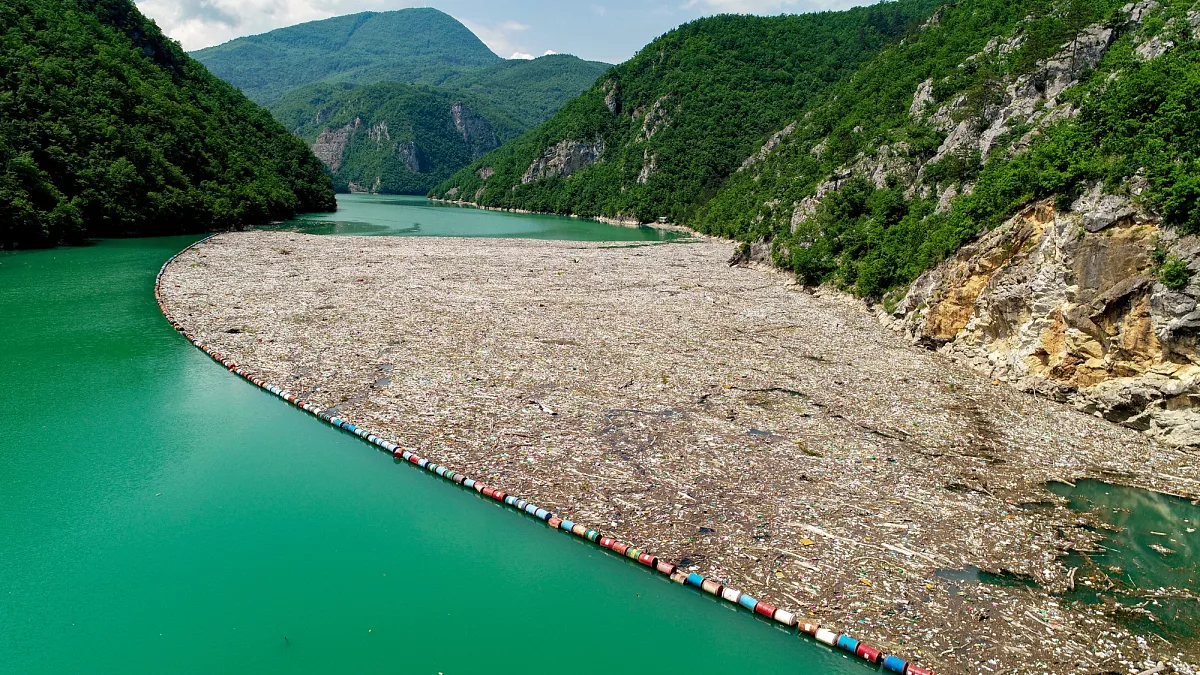
\includegraphics[width=0.6\textwidth,frame]{drina_waste}
	\caption{A drinai hulladéksziget. Egy lebegő zsinor fogja meg a műanyagpalackokat \cite{euronews2024}}
    \label{fig:drina-floating-waste}
\end{figure}

\begin{figure}[H]
	\centering
	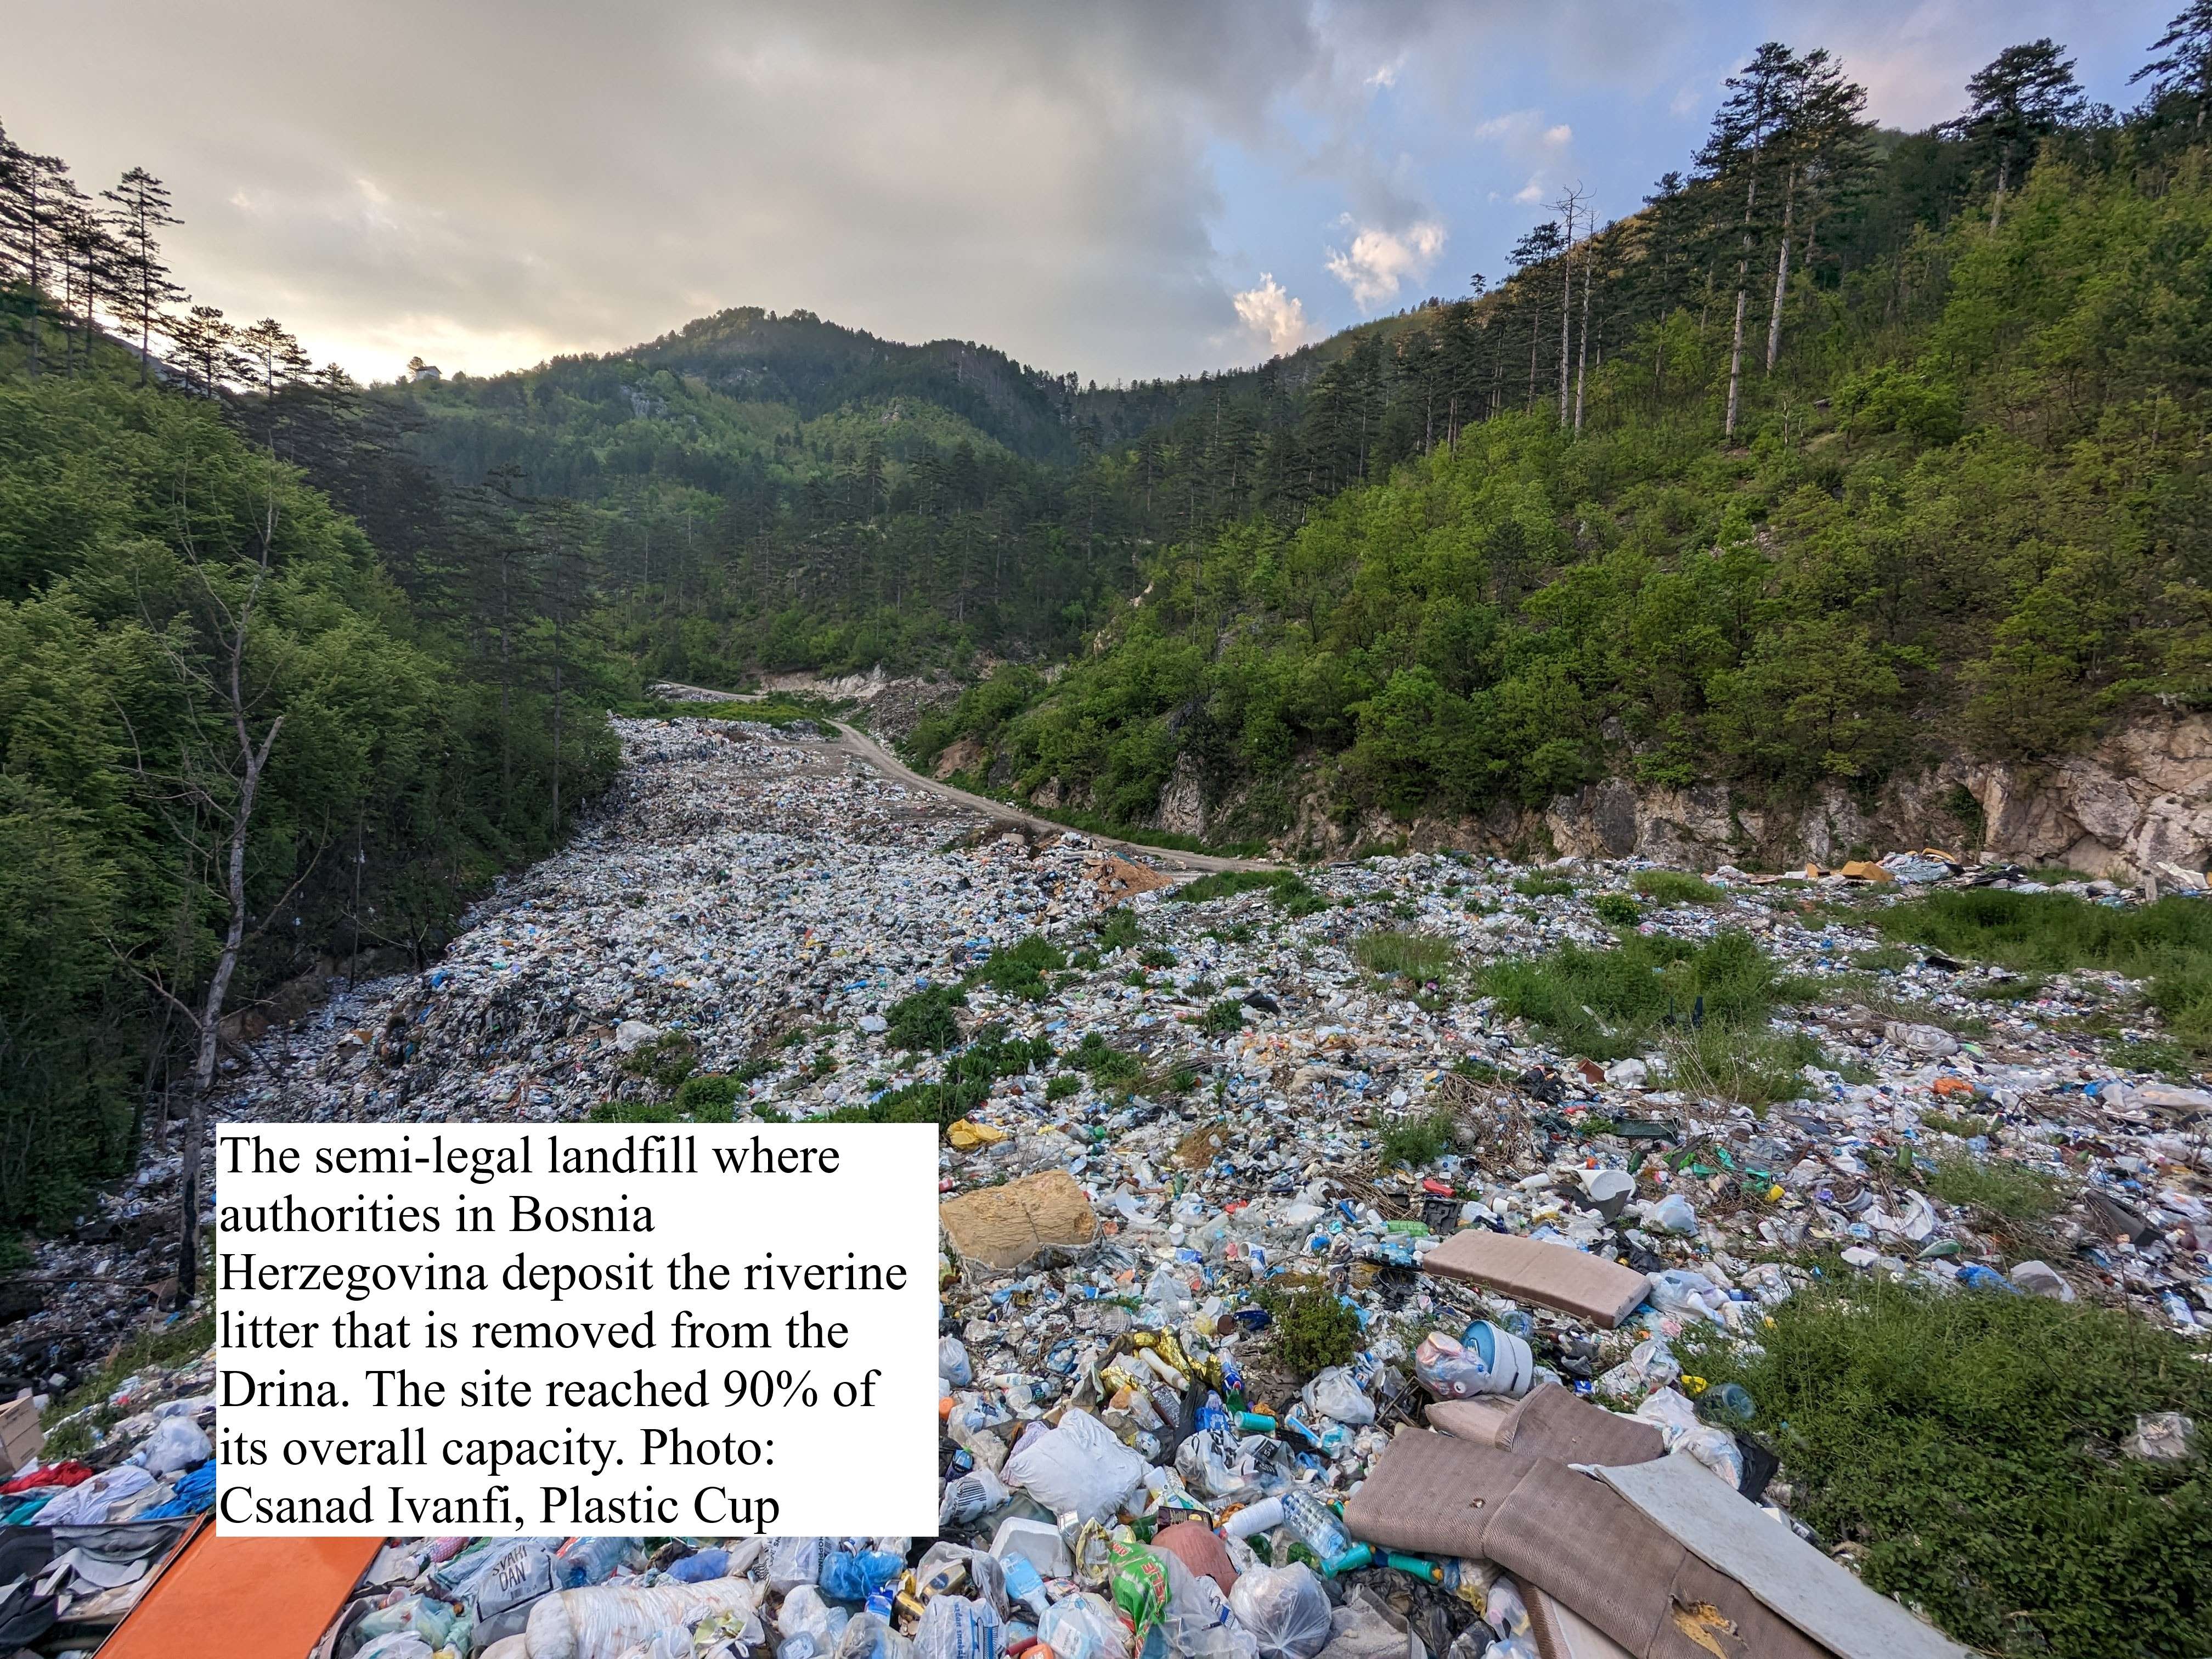
\includegraphics[width=0.6\textwidth,frame]{drina_deposit}
	\caption{A Drina melletti féllegális szemétlerakó \cite{petkupa2024}}
    \label{fig:drina-deposit}
\end{figure}

\begin{figure}[H]
	\centering
  \subcaptionbox{A teszthalmaz kézi annotációja}{
		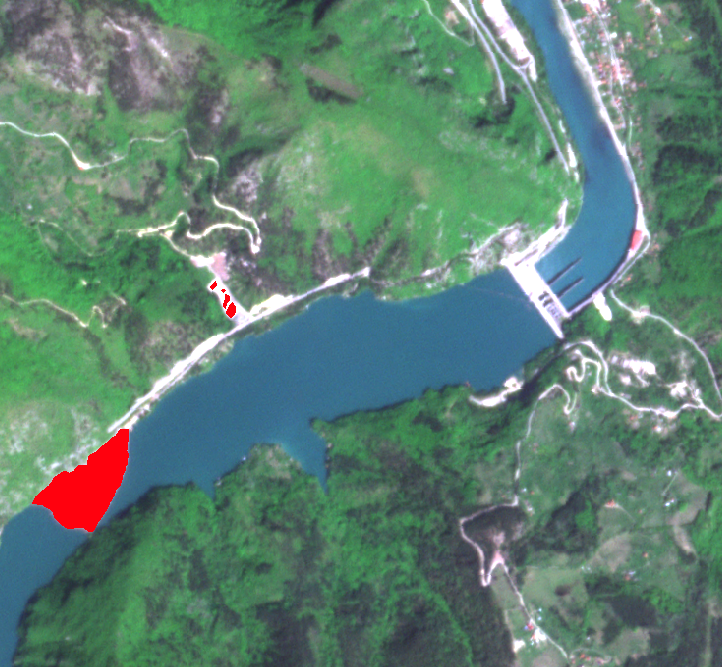
\includegraphics[width=0.45\linewidth]{drina-test}}
	\hspace{5pt}
	\subcaptionbox{A teszthalmaz annotációja a régi modellel}{
		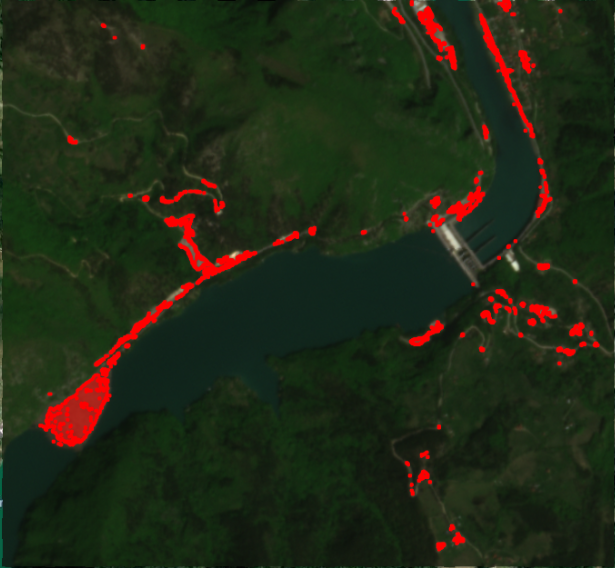
\includegraphics[width=0.45\linewidth]{drina-old}}
	\hspace{5pt}
	\subcaptionbox{A teszthalmaz annotációja az új modellel}{
		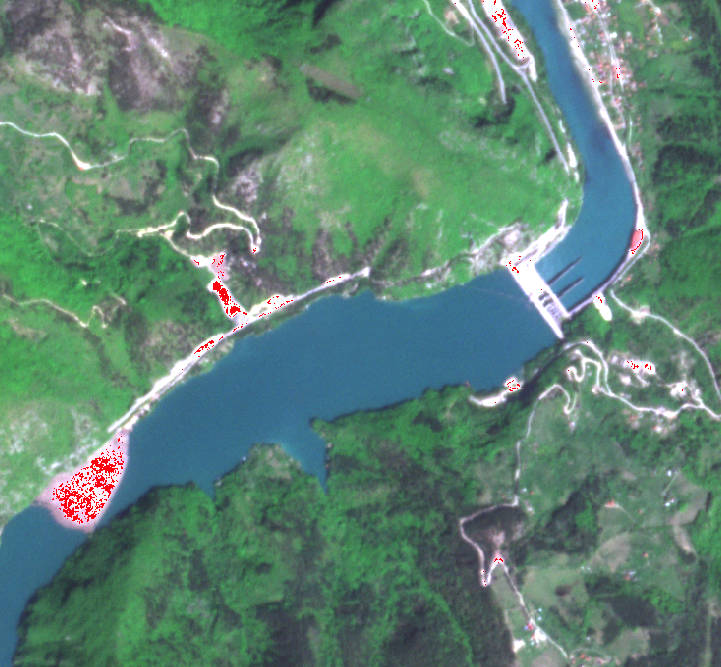
\includegraphics[width=0.45\linewidth]{drina-new}}
	\caption{Az új modell összehasonlítása a régi modellel az egyik Drinai teszt felvételen. Felvétel dátuma: 2023-05-07}
	\label{fig:old-vs-new}
\end{figure}

\section{Teljesítmény mérése}

A teszthalmaz eredményekeit a "Confusion Matrix" módszerével értékeltem ki \cite{CONGALTON199135}. Ezután ezeket az értékeket arra használtam, hogy a "Comission rate" (\ref{eq:comission-rate} képlet), "Omission rate" (\ref{eq:omission-rate} képlet), "Match rate" (\ref{eq:match-rate} képlet), illetve "Extraction rate" (\ref{eq:extraction-rate} képlet) értékeket számítsam ki \cite{Fekete2021}.

\begin{equation}\label{eq:comission-rate}
    Comission \ rate = \frac{N_{com}}{N_{ref}}
\end{equation}

\begin{equation}\label{eq:omission-rate}
    Omission \ rate = \frac{N_{om}}{N_{ext}}
\end{equation}

\begin{equation}\label{eq:match-rate}
    Match \ rate = \frac{N_{match}}{N_{ref}}
\end{equation}

\begin{equation}\label{eq:extraction-rate}
    Extraction \ rate = \frac{N_{ext}}{N_{ref}}
\end{equation}

$N_{com}$, $N_{om}$, $N_{match}$, $N_{ext}$, $N_{ref}$, rendre a false positive, false negative (A mátrix mellékátlói), true positive (A mátrix főátlója), a modell által detektált pozitív, illetve a referencia adatokban található positív értékek. Összehasonlítottam az új modell teljesítményét a régi modell teljesítményével. A \ref{tab:old-vs-new} táblázatból látható a két modell teljesítményének az átlaga a három felvételen.

\begin{table}[H]
	\centering
	\begin{tabular}{ | p{0.33\textwidth} | p{0.33\textwidth} | p{0.33\textwidth} | }
		\hline
		\textbf{Mérés azonosító} & \textbf{Régi modell átlagai (\%)} & \textbf{új modell átlagai (\%)} \\
		\hline \hline
		Comission Rate & 63.67 & 28.13 \\
		\hline
		Omission Rate & 26.21 & 70.67 \\
		\hline
		Match Rate & 73.79 & 29.32 \\
		\hline
        Extraction Rate & 208.18 & 41.31 \\
		\hline
	\end{tabular}
	\caption{A régi modell és az új modell teszteredményei átlagolva}
	\label{tab:old-vs-new}
\end{table}

Az új modell egy jóval kisebb false postive aránnyal rendelkezik mint a régi modell, de cserében a false-negative arányok is nagyok. Ennek oka a \ref{fig:old-vs-new} ábrából látható, hiszen a régi modell sokkal több pontot detektál a hulladékszigeten, míg az új modell kevesebb pontot detektál, de továbbra is nagy mértékben megtalálja a hulladékszigetet. Illetve a \ref{ch:test-set} fejezetben is tárgyaltam, hogy a szárazföldi hulladéklerakót a folyó mellett az új modell már megtalálja, míg a régi nem találja meg. Tekintve arra, hogy a match rate a true positive-al arányos, és az Extraction rate az összes pozitive-al arányos, ezek az értékek is kisebbek lesznek, mint a régi modell értékei.

\section{Főkomponens analízis teljesítménye}
\label{ch:pca-performance}

A \ref{ch:pca-methodology} fejezetben részletezett főkomponens analízis módszert is összehasonlítottam az új modell teljesítményével, a Confusion Matrix módszerének segítségével. A \ref{fig:pca-vs-no-pca} ábrából látható, hogy a főkomponens analízissel tanított modell sokkal jobban ki tudja szűrni a vízfelszínen kialakuló zajt. Az is látható, hogy a főkomponens analízissel kombinált Random Forest is hasonlóan tudja detektálni a hulladékkal szennyezett területeket.

\begin{figure}[H]
	\centering
  \subcaptionbox{A teszthalmaz kézi annotációja}{
		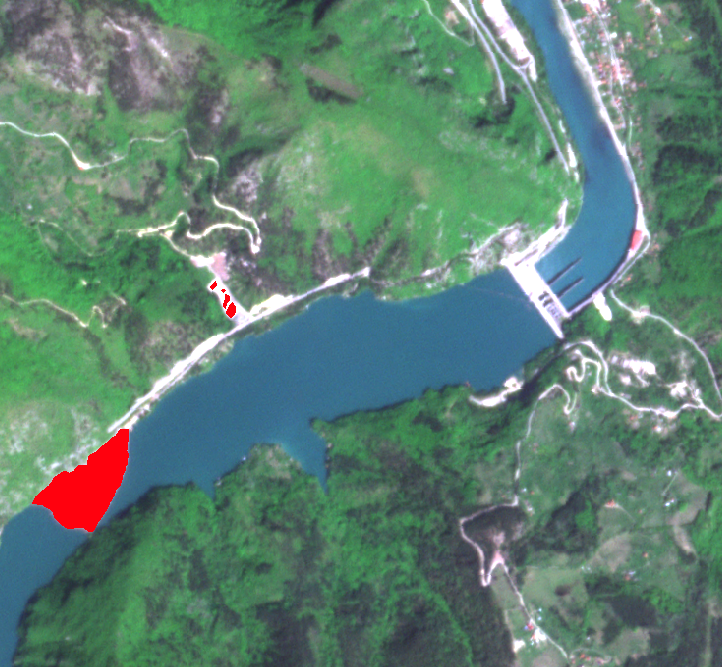
\includegraphics[width=0.45\linewidth]{drina-test}}
	\hspace{5pt}
	\subcaptionbox{A teszthalmaz annotációja az új modellel}{
		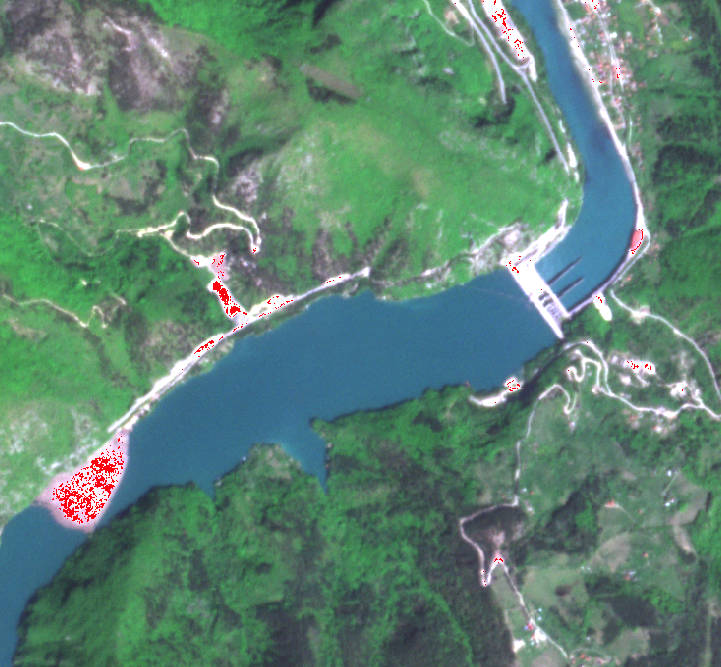
\includegraphics[width=0.45\linewidth]{drina-new}}
	\hspace{5pt}
	\subcaptionbox{A teszthalmaz annotációja az új modellel, PCA segítségével}{
		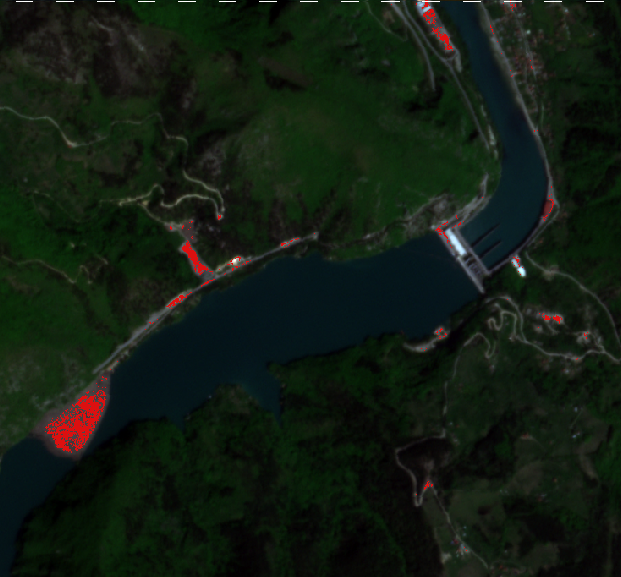
\includegraphics[width=0.45\linewidth]{drina-with-pca}}
	\caption{Az új modell összehasonlítása a PCA-val tanított modellel az egyik Drinai teszt felvételen. Felvétel dátuma: 2023-05-07}
	\label{fig:pca-vs-no-pca}
\end{figure}

A \ref{tab:pca-vs-no-pca} táblázatban összesítem a főkomponens analízis mutatóit. A táblázatból leolvasható, hogy míg a főkomponens analízis picivel nagyobb false positive aránnyal rendelkezik, egyben kisebb false negative aránnyal rendelkezik. Ráadásul a felvételeken készülő zajt sokkal jobban kezeli, amint a \ref{fig:classification-pca-vs-no-pca} ábrából is látható. A főkomponens analízissel betanított modell sokkal jobban tudta detektálni a vizet a folyón, mint a főkomponens analízis nélküi modell.

\begin{table}[H]
	\centering
	\begin{tabular}{ | p{0.33\textwidth} | p{0.33\textwidth} | }
		\hline
		\textbf{Mérés azonosító} & \textbf{PCA-val tanított modell átlagai (\%)} \\
		\hline \hline
		Comission Rate & 39.01 \\
		\hline
		Omission Rate & 65.00 \\
		\hline
		Match Rate & 34.99  \\
		\hline
        Extraction Rate & 65.25 \\
		\hline
	\end{tabular}
	\caption{A főkomponens analízissel betanított modell teljesítményének az átlagai}
	\label{tab:pca-vs-no-pca}
\end{table}

\begin{figure}[H]
	\centering
  \subcaptionbox{Drina műholdfelvétele}{
		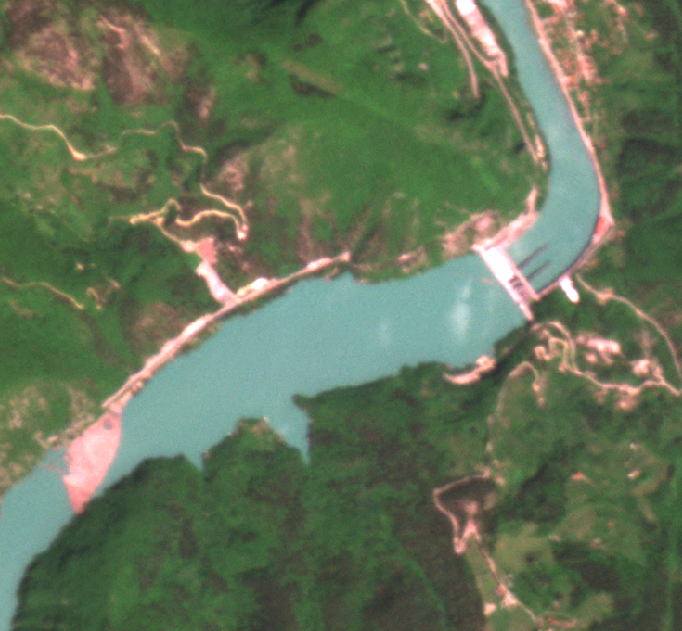
\includegraphics[width=0.45\linewidth]{drina20230521}}
	\hspace{5pt}
	\subcaptionbox{A PCA nélküli modell címkézése a Drinán}{
		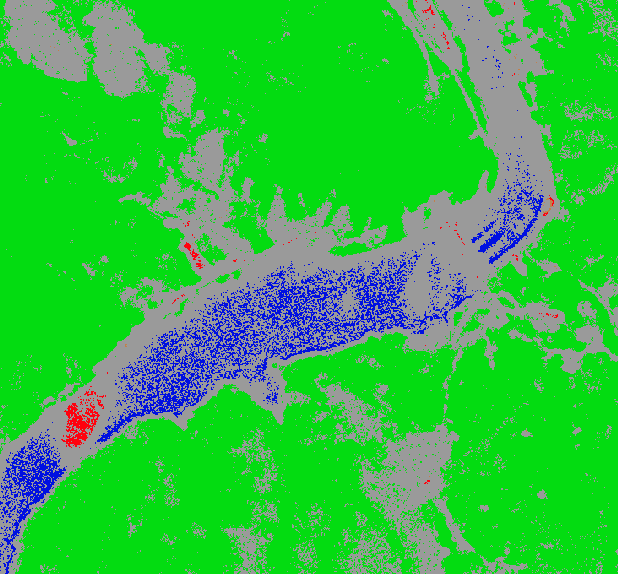
\includegraphics[width=0.45\linewidth]{drina-classification-no-pca}}
	\hspace{5pt}
	\subcaptionbox{A PCA-val betanított modell címkézése a Drinán}{
		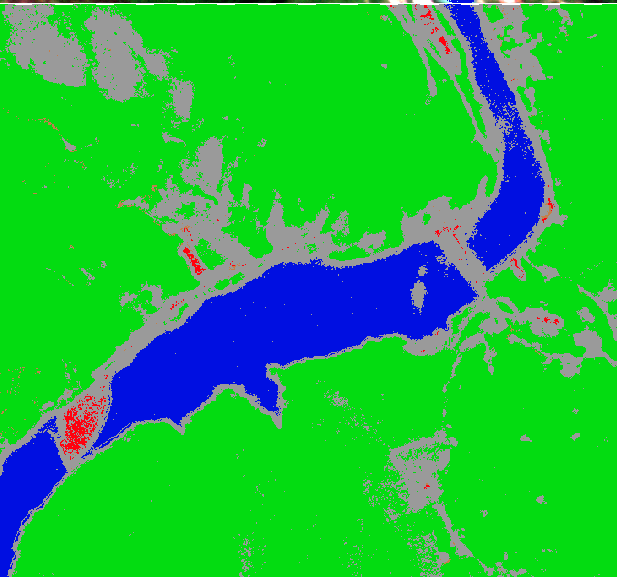
\includegraphics[width=0.45\linewidth]{drina-classification-with-pca}}
	\caption{A főkomponens analízissel betanított modell osztályozásának össszehasonlítása a PCA nélkül betanított modellel. Felvétel dátuma: 2023-05-21}
	\label{fig:classification-pca-vs-no-pca}
\end{figure}

\section{Vízmaszkolás}

Az egyik kihívás a hulladékdetektálásban a nagy lefedettségű területek feldolgozása. A kutatásunk célja a folyók közelében található hulladékkal szennyezett területeknek a detektálása, így a folyóktól távolabbi területeket érdemes kivágni a gyorsabb osztályozás érdekében. Az egyik hosszútávú cél az, hogy hosszabb folyószakaszokon is lehessen futtatni a Random Forest modellt, úgy, hogy az osztályozás elfogadható futási időn belül történjen meg.
\todo{hogy hivatkozhatok itt a laborban meglevő munkára, anélkül, hogy saját eredményként tűntessem fel?}  